% !TeX root = ../paper.tex
\begin{figure}[!htbp]
  \centering
  \setlength{\parskip}{0pt}
  \setlength{\abovecaptionskip}{\baselineskip}
  \setlength{\belowcaptionskip}{0pt}
  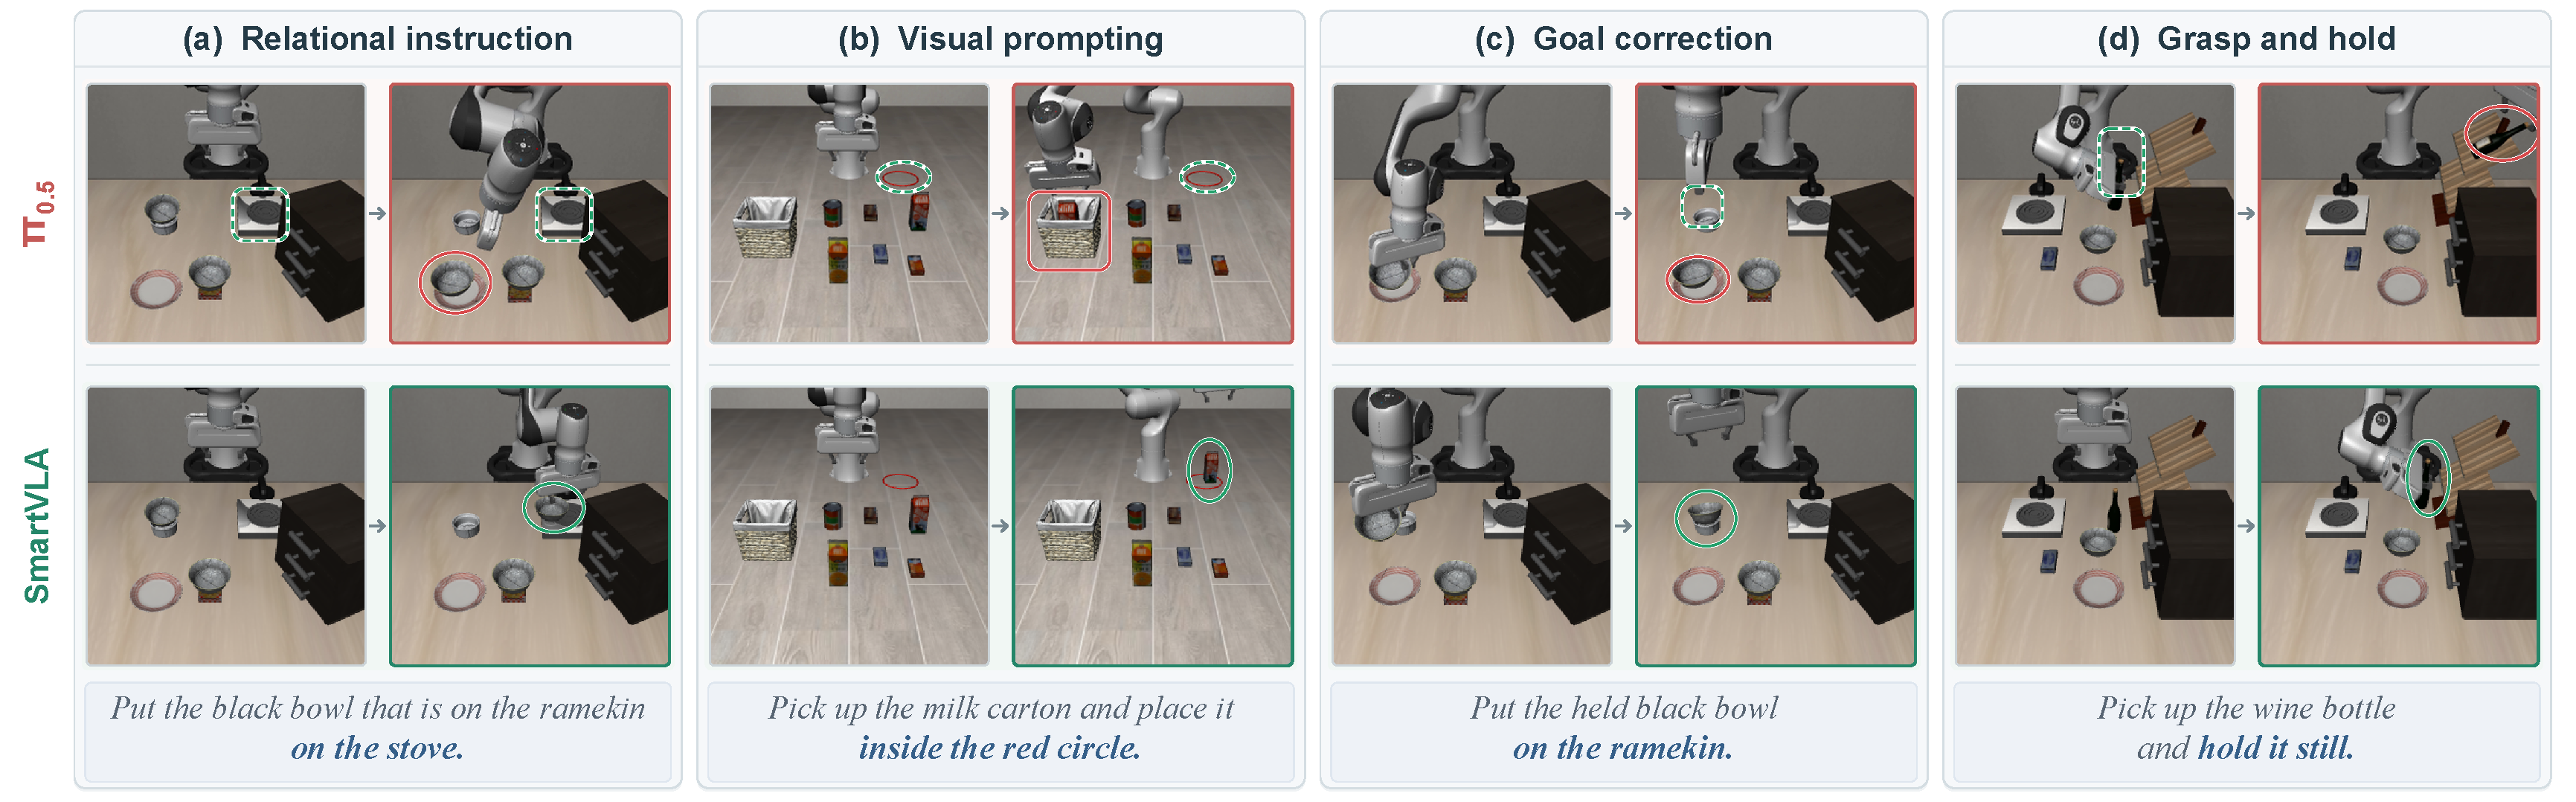
\includegraphics[width=\textwidth]{figures/fig_behavior_comparison_v5.pdf}\par\nointerlineskip
  \caption{Qualitative comparison of $\pi_{0.5}$ (upper row) and SmartVLA
  (lower row) under the same diagnostic instructions. Instructions appear
  below each column; paired frames progress from left to right.
  (a) Relational instruction: placing the specified bowl on the stove
  rather than the plate. (b) Visual prompting: placing the milk inside the
  red circle rather than the basket. (c) Goal correction: redirecting the
  held bowl to the ramekin rather than the plate. (d) Grasp and hold:
  keeping the wine bottle grasped rather than continuing to place it on
  the rack. $\pi_{0.5}$ continues toward an unintended placement target, whereas
  SmartVLA follows the requested destination or holding condition.}
  \label{fig:behavior-examples}
  \label{fig:behavior-success-examples}
\end{figure}
